\documentclass[runningheads]{llncs}

\usepackage[T1]{fontenc}
\usepackage{graphicx}
\usepackage{url}

\begin{document}

\title{What Google Knows: Measuring Telemetry and Identifier Exposure Across Privacy-Focused Android Operating Systems}

\titlerunning{Measuring Privacy Across Privacy-Focused Android Distributions}

\author{Bruno Mircevski\inst{1}\orcidID{0009-0007-1008-6708} \and
Krzysztof Jurczuk\inst{1}\orcidID{0000-0001-6469-1769}}

\authorrunning{B. Mircevski et al.}

\institute{Faculty of Computer Science, Bialystok University of Technology, Wiejska 45a, 15-351, Bialystok, Poland}

\maketitle

\begin{abstract}
This paper presents a comparative analysis of user privacy in Android operating systems through network traffic inspection. Using a controlled man-in-the-middle setup and traffic decryption techniques, six Android systems were evaluated: stock Android (GMS), GrapheneOS, iod\'eOS, and three variants of LineageOS (stock, Gapps, microG). While prior work focuses on applications or stock Android across device manufacturers, this study investigates alternative Android distributions designed with privacy as a primary objective. We examined outbound connections, transmitted identifiers, and network traffic patterns to assess the impact of integrated Google services on user privacy. Our findings demonstrate that stock Android maintains the most communication with Google servers, transmitting identifiers and metadata even when the device is not actively in use. In contrast, all privacy-focused systems minimize unsolicited traffic and offer stronger user control. These results provide practical insights into how alternative Android distributions can improve user privacy without sacrificing core functionality, highlighting the potential of open-source ecosystems as viable, privacy-respecting alternatives to Google-dependent mobile environments.

\keywords{Android \and Privacy \and Network traffic}
\end{abstract}

\section{Introduction}
Android is the dominant mobile operating system and acts as a primary gateway to the digital world for billions of users. It is crucial for the core operating system to be a reliable, stable and trustworthy platform that allows users to run applications and services of their choice. While third-party application privacy has been widely studied \cite{appDataCollection1,appDataCollection2,appDataCollection3,appDataCollection4}, less attention is typically paid to the operating system layer and to privileged service frameworks that silently enable additional functionality. Standard unprivileged applications are subject to the Android permission model, although some attempt to circumvent these restrictions in creative ways \cite{appDataCollection5Circumvention,appDataCollection6Circumvention}. In contrast, privileged system applications operate with higher access to the device and OS, which makes their actions harder to understand and control. Most user-facing privacy controls focus on applications and permissions, yet a substantial amount of data exchange can occur at lower layers, through OS services, vendor components, and integrated Google services. This work therefore compares the network behavior of multiple Android distributions and their preinstalled/privileged system components under controlled, reproducible conditions.

\subsection{Android dependency on privacy-threatening services}
While the Android core is the Android Open Source Project (AOSP), most consumer devices include additional proprietary components layered on top. They are often implemented as privileged system applications and services to provide baseline functionality such as push notifications, location assistance, application distribution/updates, device integrity checks, and many others. Users and application developers commonly assume their presence and availability by default. 

These components exist for a practical reason. Centralized services can significantly improve usability and efficiency, for example by reducing battery drain compared to per‑application background connections, and by providing faster, more accurate location through fused network and sensor-based methods. However, this design also tightly couples many functions into a single service stack. Enabling useful capabilities may implicitly enable others that a user would not choose, such as advertising identifiers, telemetry, and behavioral tracking. In practice, the result is a large proprietary bundle that is difficult to audit and decompose into only the features a user actually wants.

On Android, these baseline capabilities are most commonly delivered through GMS (Google Mobile Services). Because Google’s business model is strongly advertising-driven, many users may be unwilling to entrust this provider with broad access to their devices and data. In principle, users should be able to choose which services they rely on and have confidence that these choices are enforced by the platform’s permission and isolation mechanisms. This demand for transparency and controllability motivates alternative approaches such as microG\footnote{\url{https://github.com/microg/GmsCore/wiki}} and GrapheneOS sandboxed Google Play\footnote{\url{https://grapheneos.org/usage#sandboxed-google-play}}. These solutions aim to preserve device functionality and application compatibility while reducing privilege and improving user control over Google-related components.

\subsection{Privacy-focused Android operating systems}
Privacy-focused Android operating systems are distributions derived from AOSP that aim to reduce data exposure at the OS level. They achieve this by limiting preinstalled privileged components, tightening default settings, and providing more transparent controls over permissions and network access. In contrast to stock Android (the factory system shipping with Google Mobile Services enabled by default), privacy-oriented systems minimize background communication, restrict persistent identifiers, and strengthen user enforcement mechanisms over non-essential components.

In this work we focus on three representative approaches: GrapheneOS, iod\'eOS, and three variants of LineageOS (stock, Gapps, microG). GrapheneOS\footnote{\url{https://grapheneos.org/}} prioritizes a hardened security model and strong isolation. Google components are not included by default, but can be installed in a dedicated sandboxed mode as ordinary applications, without the special privileges they typically hold on factory systems. This design targets improved containment and user control while preserving high compatibility when the user decides to install Google services. GrapheneOS also improves low-level security, for example by replacing Android’s default memory allocator with its own hardened implementation to make memory corruption exploitation harder \cite{graphene-hardened}.

LineageOS\footnote{\url{https://lineageos.org/}} provides a lightweight, broadly supported AOSP-based system with minimal preinstalled software and extensive device compatibility. It can be deployed in multiple configurations: without Google services, with proprietary Google Play Services (Gapps\footnote{\url{https://mindthegapps.com/}}), or with microG\footnote{\url{https://lineage.microg.org/}} as an open-source reimplementation of key Google components. These configurations represent different trade-offs between privacy, compatibility, and reliance on proprietary services.

Finally, iod\'eOS\footnote{\url{https://iode.tech/iodeos/}} is a privacy-oriented distribution based on LineageOS that combines a de-Googled baseline with additional privacy features and preconfigured app ecosystem choices, shipping with microG. For completeness, CalyxOS\footnote{\url{https://calyxos.org/}} and /e/OS\footnote{\url{https://e.foundation/e-os/}} follow a similar privacy-oriented direction (AOSP-based, microG-enabled, and designed for practical daily use). They were considered for the study, but were excluded because they had not shipped Android 16 builds during the measurement period.
\\
\\
\noindent Our main contributions are as follows: 
\begin{itemize}
	\item We present a comparative network-level privacy analysis of six Android system configurations, including stock Android, GrapheneOS, iod\'eOS, and multiple LineageOS variants, covering a broad spectrum of Google service integration models.
	\item We provide, to the best of our knowledge, the first systematic empirical comparison between privileged Google Mobile Services (GMS), sandboxed Google Play Services in GrapheneOS, and open-source replacements such as microG under comparable conditions.
	\item We design a controlled real-device measurement methodology for modern Android systems (Android 16), combining traffic interception, TLS decryption where possible, and realistic user scenarios including setup, idle operation, and basic tasks.
	\item We quantify how alternative Android distributions reduce unsolicited background communication, limit identifier exposure, and improve user control compared to stock Android, while preserving core functionality.
\end{itemize}

The rest of the paper is structured as follows. Section 2 reviews related work concerning network traffic analysis and Android privacy. Section 3 details the experiment design, including the hardware, software, and specific measurement scenarios utilized in our study. Section 4 presents the evaluation results, highlighting data usage across configurations, analysis of specific packet and data obtained from Google Takeout. Section 5 discusses the broader implications of these findings, along with study limitations. Finally, Section 6 concludes the paper and outlines potential directions for future research.

\section{Related work}

Prior work has established that Android privacy risks arise not only from user-installed applications but also from the operating system and its preinstalled components \cite{android-os-snooping2021,android-os-snooping2023,google-dialer-messages,cookies-identifiers2025,google-data-collection2018}. Privacy-focused Android distributions have gained popularity as alternatives to stock vendor firmware, yet they remain comparatively understudied in the measurement literature. Consequently, there is limited empirical understanding of what practical privacy and control benefits different Android distributions provide to users.

To address this gap, an OS-level measurement study compares user privacy of several vendor-customized Android variants with two open-source distributions \cite{android-os-snooping2021}. It reports that all tested stock/vendor builds transmit substantial data to OS vendors and third parties. Data transmission occurs even when the handset is idle, and collection is persistent without an effective opt-out. In contrast, the privacy-focused open-source /e/OS exhibits minimal data transmission. LineageOS still shows substantial communication with Google, because it was evaluated with proprietary Google components (Gapps) present. This distinction is important for studies like ours that evaluate multiple distributions and configurations (including variants with and without integrated Google services). The presence of Google system components can dominate observed traffic and shape the overall privacy profile.

Another work focusing specifically on OEM telemetry further shows that Samsung, Xiaomi, Huawei and Realme make extensive use of long-lived hardware identifiers \cite{android-os-snooping2023}. They also collect a list of installed apps and analytics data, sometimes even in connections that should not require persistent identifiers, enabling straightforward linkage to a user’s identity when an OEM account is used.

Related work by the same authors analyzes telemetry from two core Google system applications: Google Messages and Google Dialer, by decrypting and decoding the logging channels that forward data to Google \cite{google-dialer-messages}. The study reports that these applications disclose sensitive communication metadata, including when SMS messages and calls are sent or received, with timestamps and call durations. Google collects a hash derived from message content that can uniquely identify messages and link participants. Other findings show that phone numbers may be transmitted and events are tagged with persistent identifiers such as the Android ID, undermining anonymity and leaving users with no effective opt-out. Overall, the results suggest that even basic default communication apps on stock Android cannot be assumed to be trustworthy from a privacy perspective.

Complementing OS-level telemetry measurements, a recent study focuses specifically on what preinstalled Google components persistently store on-device \cite{cookies-identifiers2025}. It shows that Google’s role in Android privacy extends beyond outbound traffic. Google Play Services, Play Store and other bundled Google applications receive and store multiple cookies, advertising-related identifiers, and tracking links. Some data persists even after a factory reset and is transmitted when the user has not opened Google applications, with no dedicated consent prompt or practical opt-out. The study highlights that the Google Android ID is a persistent identifier provisioned early and widely reused in subsequent Google connections. It also documents how additional tokens and cookies can be stored and later transmitted alongside telemetry or analytics events. These findings support that Google components play a central role in Android privacy. They shape device identification and data handling independently of user-installed applications.

A broader report \cite{google-data-collection2018} examines Google's data collection from a wider perspective. It describes data collection as an ecosystem across platforms, applications and advertising services, not as a single feature of Android. It distinguishes "active" data sharing (when users directly use Google products) from "passive" collection that happens in the background. It highlights the risk of Google's tracking and analytics components embedded in many third-party applications and websites. The report argues that these different data sources can be combined to build detailed user profiles. It demonstrates that "pseudonymous" identifiers can still be linked back to user accounts when they appear together in the same workflows.

Prior work consistently indicates that Google is a dominant driver of privacy-relevant data flow on Android. It enables persistent device identification, background telemetry and cross-context linkage between application usage, web activity and advertising infrastructure. At the same time, the literature suggests that meaningful reductions in unsolicited communication are possible when Google components are absent or replaced with open-source variants \cite{android-os-snooping2021}. Alternative configurations and distributions remain less widely deployed, less familiar to typical users, and comparatively under-explored in reproducible measurement studies. This motivates systematic comparisons of stock systems and privacy-oriented alternatives, which we perform in this work to quantify privacy improvements and their trade-offs. While emulator-based setups enable highly reproducible traffic capture \cite{parrot2025}, we used a physical device to analyze behavior in a real environment, at the cost of reduced control and reproducibility.

\section{Experiment design}

\subsection{Hardware and software}

We used a single Google Pixel 6a device (codename \textit{bluejay}) to install and evaluate the studied Android distributions. This model was chosen due to its broad compatibility with alternative operating systems. All tested builds are based on Android 16 and were obtained in December 2025. The BP4A and BP2A baseline differ due to LineageOS and iod\'eOS slower update cycle.

\begin{itemize}
	\item Stock Android: \texttt{BP4A.251205.006};
	\item LineageOS: \texttt{lineage-23.0-20251206} (\texttt{BP2A.250805.005});
	\item LineageOS for microG: \texttt{lineage-23.0-20251203-microG} (\texttt{BP2A.250805.005});
	\item GrapheneOS: \texttt{2025121200} (\texttt{BP4A.251205.006});
	\item iod\'eOS: \texttt{7.0-20251129-bluejay} (\texttt{BP2A.250805.005}).
\end{itemize}

\begin{figure}
	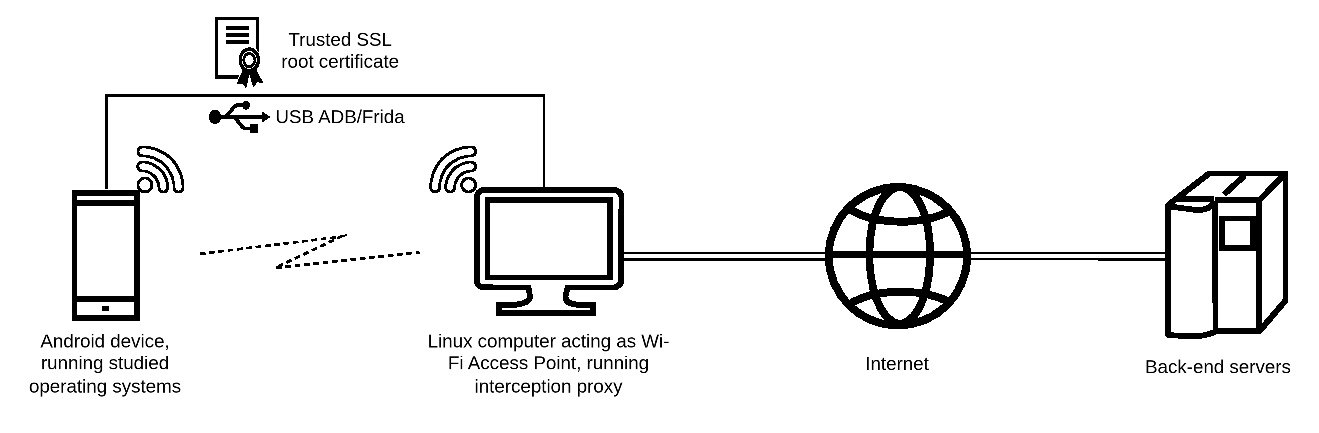
\includegraphics[width=\textwidth]{devices.eps}
	\caption{Measurement setup. The Android device running the investigated operating systems is configured to access the Internet using Wi-Fi. The access point is hosted on a Linux computer, running traffic interception and capture software. A custom system certificate is installed on the phone using root access. A USB connection is used for ADB/Frida communication.} \label{fig-devices}
\end{figure}

Android traffic analysis is limited by encryption, certificate pinning, and anti-tamper mechanisms. We captured traffic through a controlled MITM Wi-Fi gateway and intercepting proxy. QUIC over UDP/443 was blocked to force TCP-based TLS, which may alter fallback behavior and is itself remotely observable. The proxy CA was installed as a system certificate using root, and runtime unpinning was attempted where needed and possible. Full packet captures were compared across distributions, but coverage remained incomplete. Thus, a negative finding means ``not observed on decrypted channels,'' not ``not transmitted.'' Figure~\ref{fig-devices} shows the setup.

\subsection{Threat model}

This study evaluates privacy at the operating-system layer, focusing on data transmitted by privileged system components and integrated Google services. We assume a privacy-conscious user who wants to use a smartphone for everyday tasks while limiting the exposure of personal data, persistent identifiers, and behavioral metadata to remote service providers.

We define the primary adversary as Google due to its preinstalled, privileged system components and its data-driven advertising business model, which relies on extensive data collection. Google can receive traffic initiated by the OS, retain server-side records linked to a Google account, and build long-term profiles from persistent identifiers and recurring background activity.

We do not model active on-device attackers, physical device compromise, baseband-level attacks, or the exploitation of OS vulnerabilities. Therefore, this evaluation focuses on privacy leaks from standard, intended service integrations rather than device security.

\subsection{Measurement scenarios}
Four scenarios specify Google account state, consent and permissions, and installed Google components; not all apply to every system. On GrapheneOS, sandboxed Google Play Services were installed immediately after setup. On microG systems, microG was enabled during setup when prompted or immediately afterward. Other unavailable setup steps were likewise performed as soon as possible.

\paragraph{Scenario A1: Default setup with Google account.}
The device is configured to reflect a typical user path. Google account sign-in is performed during setup (or immediately after) and default recommendations are accepted (including prompted permissions). This scenario is applicable to all systems, except LineageOS without any form of Google services.

\paragraph{Scenario A2: Minimal setup with Google account.}
This scenario retains a Google account but declines optional consents and permissions and maximizes system and account privacy settings. Because privacy-focused systems expose fewer such options, Scenario A2 was measured only on stock Android and LineageOS with Gapps; other systems used Scenario A1 only.

\paragraph{Scenario B: Minimal setup without Google account.}
The device is configured with maximum privacy in mind, avoiding Google account sign-in entirely. During initial setup, only strictly required prompts are accepted and optional data-sharing is declined. System settings are adjusted to maximize user privacy. Google components or their functional replacements remain present and enabled to preserve baseline device functionality and application compatibility, but operate without an account. This scenario is applicable to the same systems as Scenario A1.

\paragraph{Scenario C: Extremely minimal setup without Google components.}
This scenario applies only to distributions that do not bundle or enable Google services by default. It is not applicable to the official factory system, which enables Google components by default. If microG is preinstalled, it remains disabled. We did not attempt to disable Google services on stock Android, as doing so significantly degrades or breaks core system and application functionality.

\subsection{Measurement tasks}
The following tasks were performed sequentially for each scenario and captured with Wireshark.\footnote{\url{https://www.wireshark.org/}} Each system--scenario--task cell was measured once; without variance estimates, small differences and anomalies are not statistically reliable.

\paragraph{Task 0: Initial setup.}
The device was configured according to the target scenario. Network traffic capture began with the device's first Internet connection and continued until 10 minutes after setup completion.

\paragraph{Task 1: System idle.}
All pending automatic updates were allowed to install and complete. The device was rebooted to begin capture, then kept connected to the monitored network for at least 30 minutes. During this period, the device was unlocked three times and the application list was scrolled through. No applications were opened.

\paragraph{Task 2: Basic application interactions.}
Basic preinstalled applications were opened and simple actions (which should not require an Internet connection) were performed:
\begin{itemize}
	\item Settings: disable haptic feedback; toggle dark mode; check per-application battery usage;
	\item Clock: set an alarm;
	\item Files: create a folder;
	\item Contacts: create a local (on-device) contact.
\end{itemize}

Beyond direct task comparisons, we chose specific packets for detailed analysis to compare data transmission practices across different system configurations. This helped to characterize what data is sent and how. This analysis required TLS decryption via the intercepting proxy and, in some cases, runtime certificate unpinning with Frida using scripts from HTTP Toolkit.\footnote{\url{https://github.com/httptoolkit/frida-interception-and-unpinning}} Although Frida-based unpinning failed in most attempts, it was useful in some cases. Where needed, we used publicly available Protocol Buffer definitions from microG's source code\footnote{\url{https://github.com/microg/GmsCore/}} to decode payloads.

In addition to network-level observations, Google Takeout\footnote{\url{https://takeout.google.com/}} was used to download data collected by Google for test accounts. It allowed us to inspect and compare server-side data associated with running scenarios involving different implementations of Google services (stock Android, sandboxed Google Play, microG).

\section{Results}

\subsection{Data usage across operating systems and scenarios}

Total network data usage across all operating systems and applicable scenarios is presented in Figures~\ref{fig-setup-chart}--\ref{fig-apps-chart}. Traffic volume is contextual rather than a direct privacy metric, because small requests may carry identifiers while large transfers may not. To keep the results comparable and avoid dominance by bulk transfers, we excluded traffic to domains used for application and system update payload delivery (large binary downloads). However, this exclusion was not perfect, and some residual update-related traffic remains in the dataset. Generally, we expect lower network traffic in configurations with fewer Google services present.

\begin{figure}
	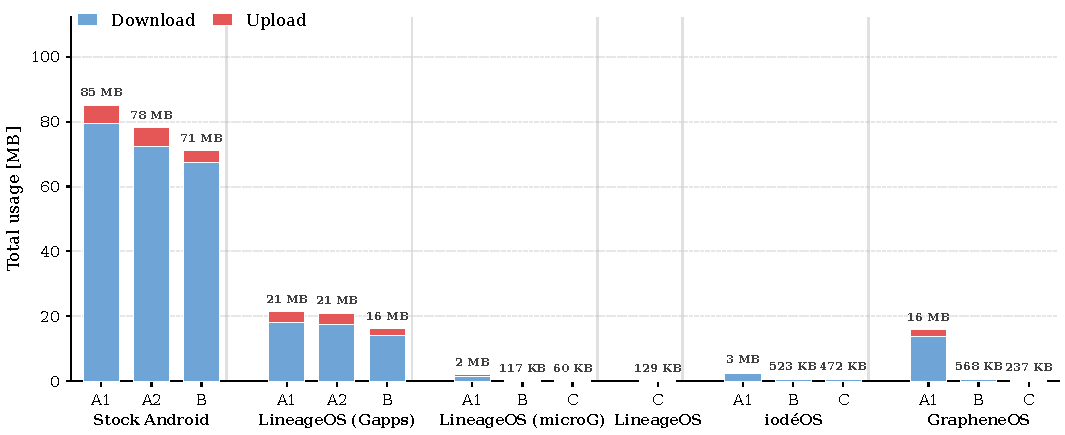
\includegraphics[width=\textwidth]{setup-data-usage.pdf}
	\caption{\textit{Task 0: Initial setup} data usage (MB). Scenario applicability varies by system (e.g., Scenario A1 requires Google services, which are absent on LineageOS).} \label{fig-setup-chart}
\end{figure}

Figure \ref{fig-setup-chart} illustrates network activity during initial device setup. As expected, stock Android shows the highest data usage (71-85 MB). The modest reductions between privacy-adjusted scenarios indicate that configuration choices provide little control over automatic updates and background activity. Configurations incorporating more Google services generate higher traffic, while de-Googled baselines demonstrate substantially reduced data exchange. LineageOS with official Google Play Services generates substantially less traffic (16-21 MB) than stock Android due to its minimal base system. However, it remains considerably higher than configurations without proprietary Google services, with the microG variant and the Google-free installation achieving notable further reductions (0-3 MB). For GrapheneOS, Scenario B demonstrates that even when sandboxed Google Play Services are installed and granted network and background permissions, they remain largely inactive when not deliberately invoked. This contrasts with the persistent background activity characteristic of integrated GMS deployments.

\begin{figure}
	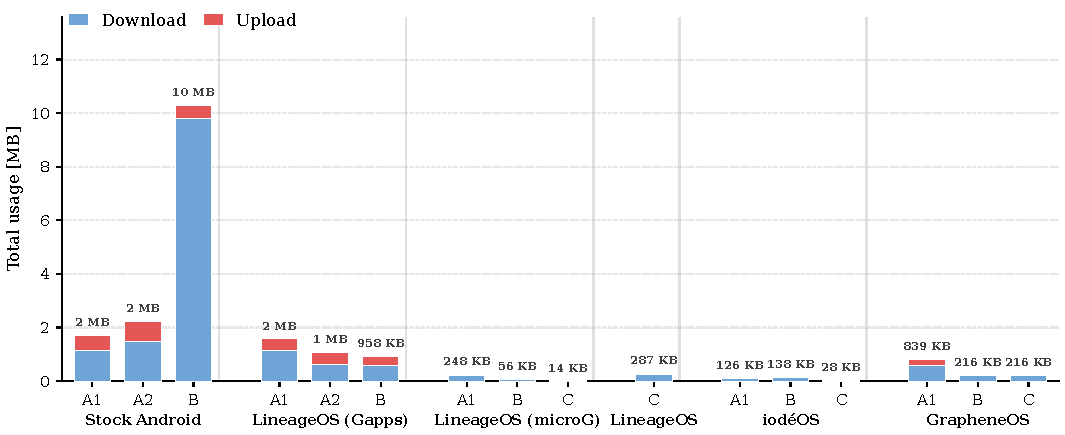
\includegraphics[width=\textwidth]{idle-data-usage.pdf}
	\caption{\textit{Task 1: System idle} data usage (MB). Scenario applicability varies by system; Scenario A2 was measured only on stock Android and LineageOS with Gapps.} \label{fig-idle-chart}
\end{figure}

Network activity observed during system idle following a reboot is presented in Figure \ref{fig-idle-chart}. Stock Android again shows the highest data usage, though Scenario B exhibits unexpectedly elevated traffic compared to both Scenario A2 and Scenario A1. This anomaly results from substantial background communication with \textit{www.gstatic.com}, likely triggered by automatic updates or other background activity during the measurement period.

LineageOS in Scenario C similarly deviates from anticipated patterns, generating more idle traffic than its microG variant. GrapheneOS exhibits nearly identical traffic in Scenarios B and C, indicating minimal background activity from sandboxed Google Play Services in these captures when not actively in use.

\begin{figure}
	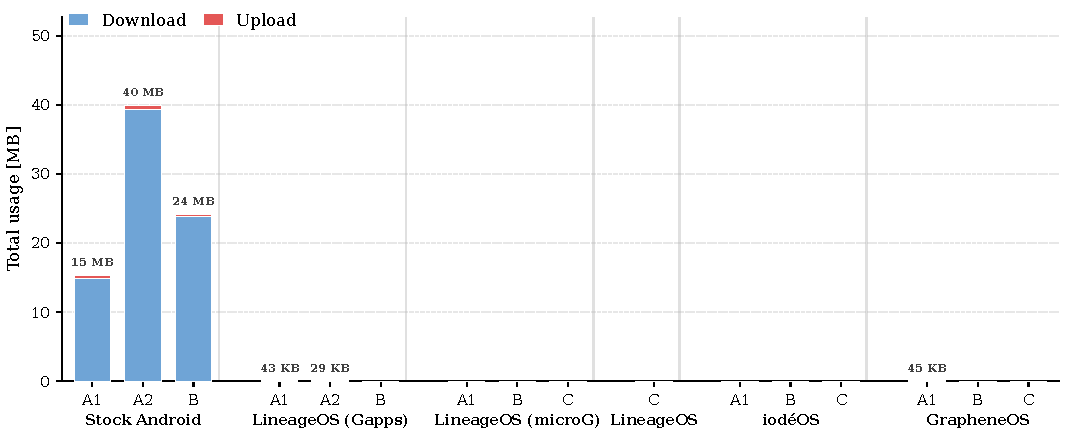
\includegraphics[width=\textwidth]{apps-data-usage.pdf}
	\caption{\textit{Task 2: Basic application interactions} data usage (MB). Scenario applicability varies by system (e.g., Scenario C is not applicable to stock Android, which bundles Google services by default).} \label{fig-apps-chart}
\end{figure}

Figure~\ref{fig-apps-chart} shows network activity during basic application interactions that should not require Internet connectivity. Stock Android dominates with substantial data usage caused mostly by uncontrolled updates. All alternative distributions demonstrate significantly lower traffic, with de-Googled configurations remaining effectively silent in the captured traffic. Notably, whenever official Google Play Services were present and a Google account was logged in, at least one request to Google infrastructure was observed.

\subsection{Domain distribution and Google dependencies}

\begin{figure}
	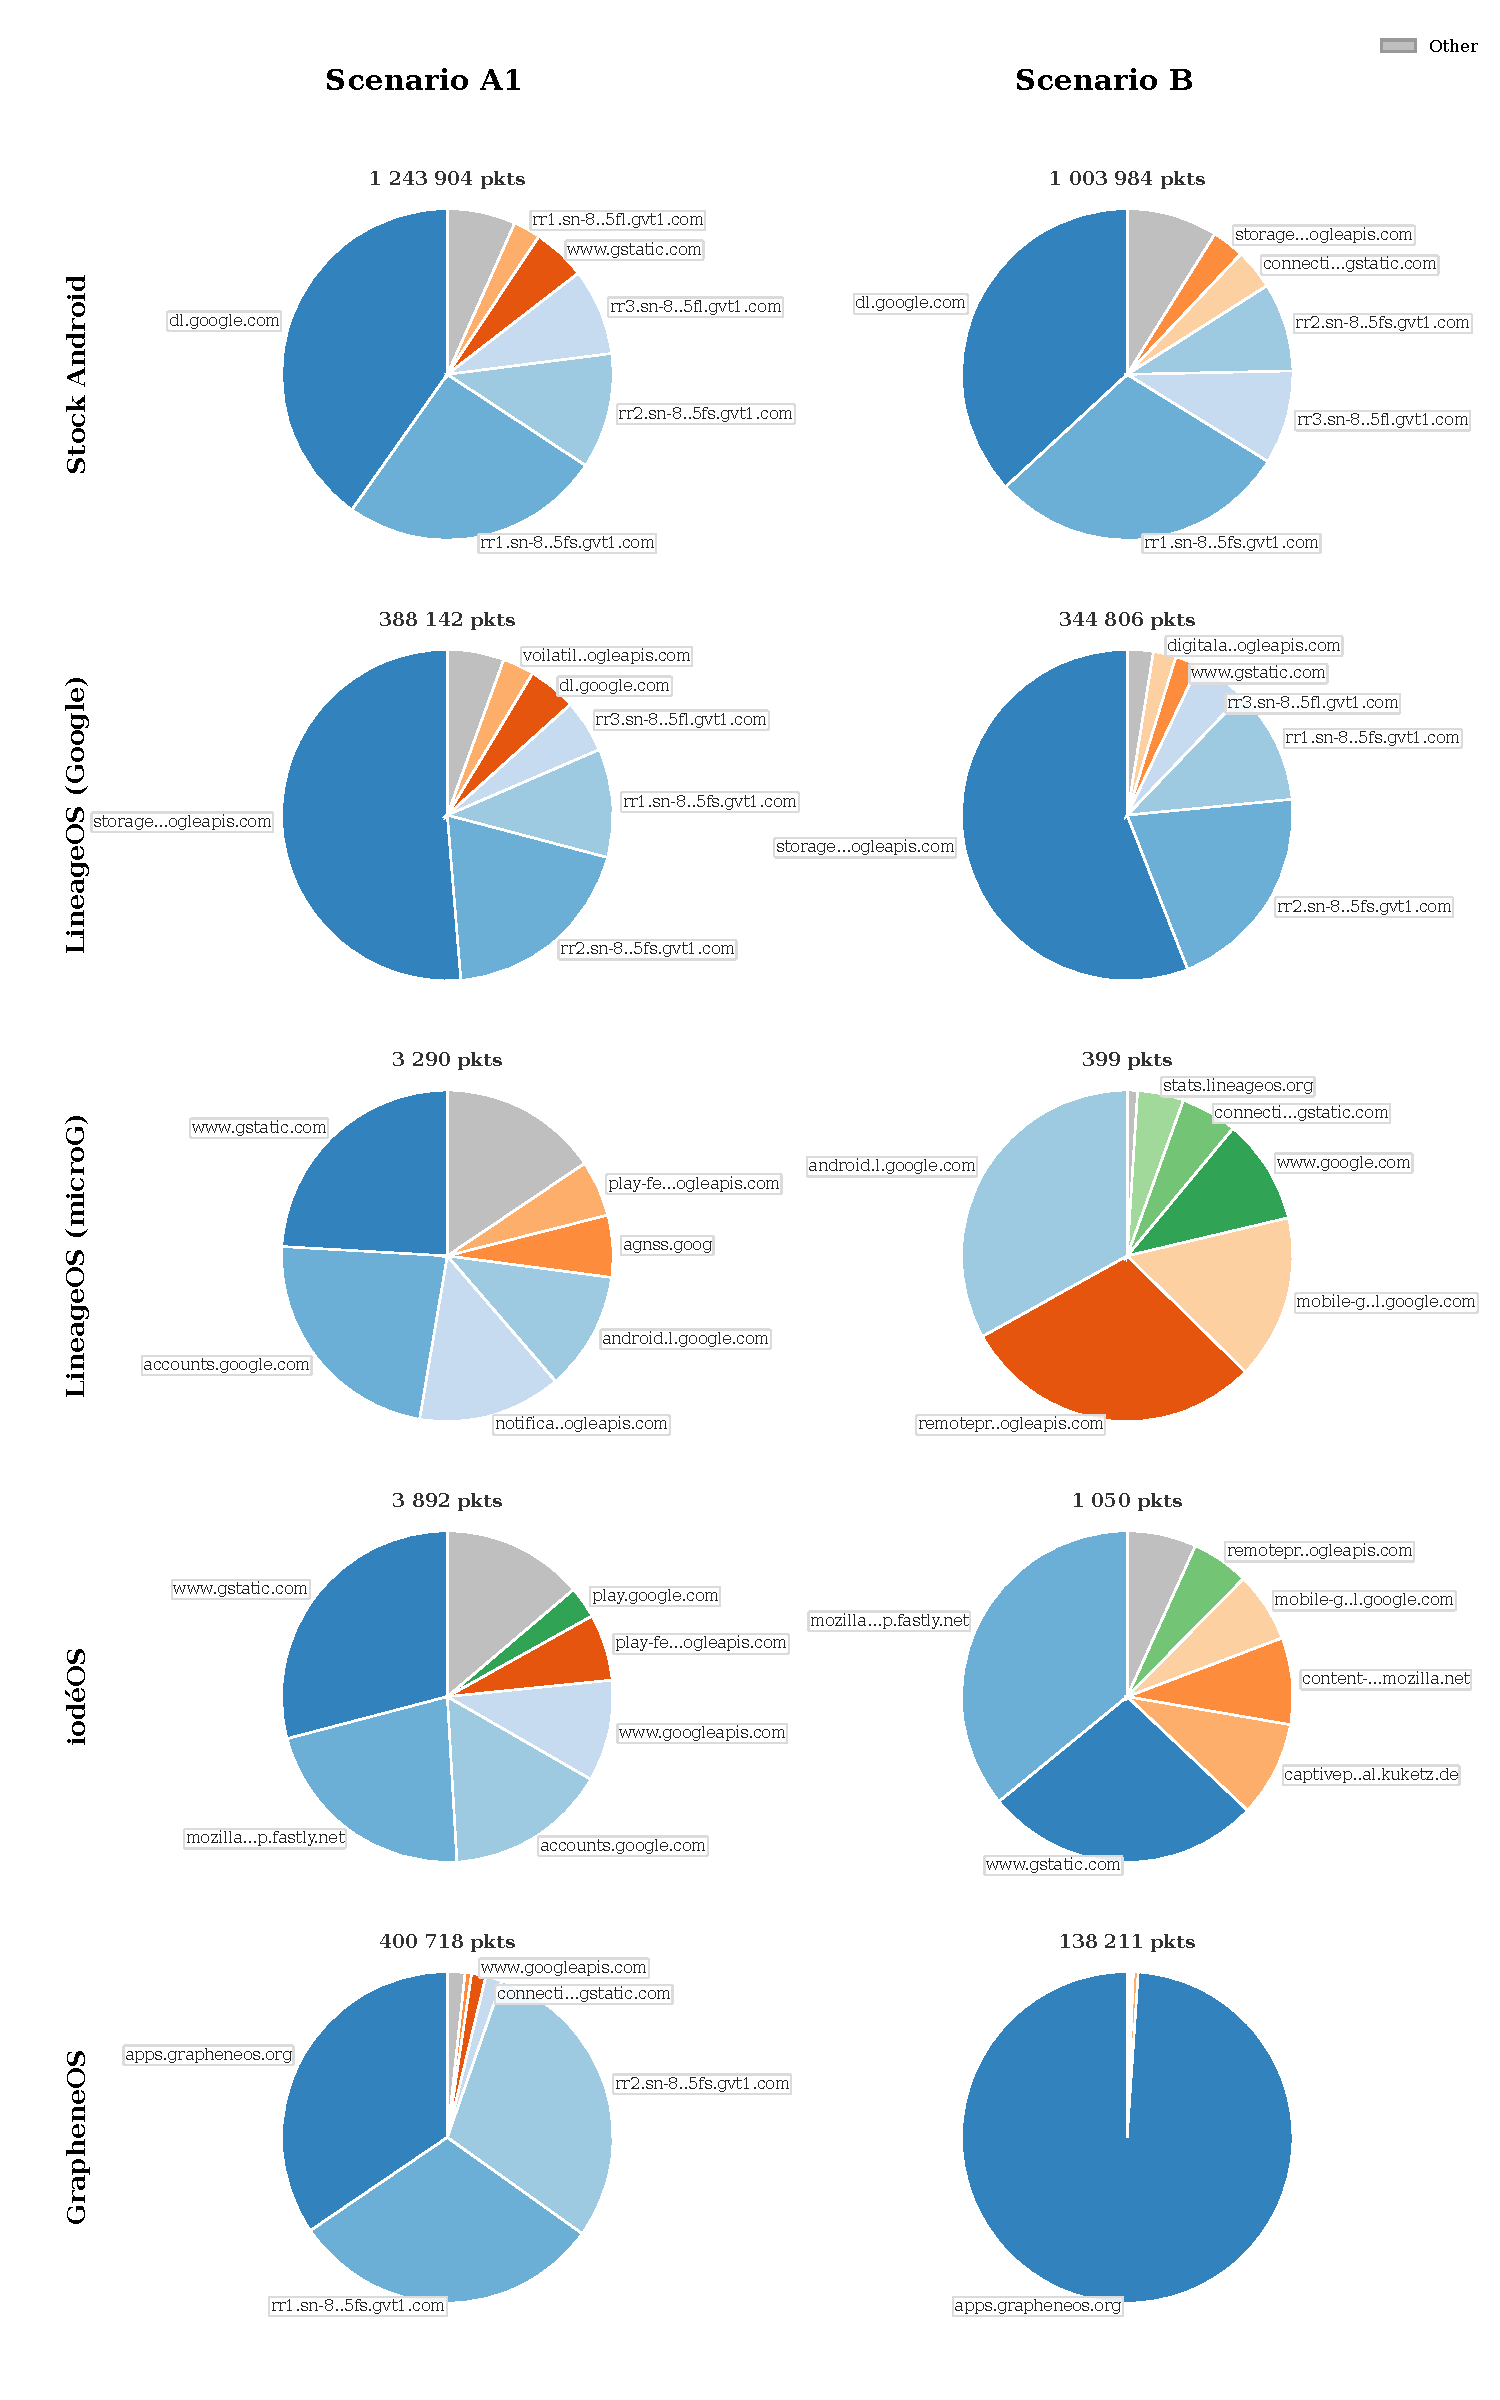
\includegraphics[width=\textwidth]{domains.pdf}
	\caption{Domain-level distribution of network packets (pkts) for scenarios A1 (with Google account) and B (without Google account, but with Google services present), aggregated over all tasks. Each pie shows the top domains by packet count for a given operating system and scenario.} \label{fig-domains-chart}
\end{figure}

Figure \ref{fig-domains-chart} presents the domain-level distribution of network traffic for Scenarios A1 and B. These scenarios were selected as the most realistic configurations, incorporating essential Google functionality while differing in account linkage and privacy-related settings. Overall traffic is dominated by large content transfers, as systems download necessary resources and updates. The totals include Google-directed and non-Google traffic, such as GrapheneOS repository downloads and iod\'eOS communication with Mozilla infrastructure. Stock Android contacts the widest range of Google domains, distributing traffic across numerous endpoints. Alternative systems show reduced Google communication, although patterns vary by design. GrapheneOS generates more requests than microG-based systems, as it downloads Google services on demand from its own application store. iod\'eOS and LineageOS with microG contact fewer Google servers overall, as microG minimizes connectivity while still enabling basic functionality.

Table \ref{tab:domains-mechanisms} shows the infrastructure dependencies for core system functions. LineageOS variants remain closest to stock Android, relying entirely on Google servers for connectivity checks, remote provisioning, and location assistance. iod\'eOS adopts an intermediate position, using independent infrastructure for connectivity checks while still depending on Google for remote provisioning and location services. GrapheneOS demonstrates the strongest de-Googling, substituting all three functions with its own or independently operated infrastructure. Both iod\'eOS and GrapheneOS expose these mechanisms through explicit system settings toggles, though GrapheneOS offers more granular control: users may choose between its independent proxy infrastructure and official Google servers for each function, with the default configured to avoid Google connections entirely.

\begin{table}
	\caption{Domains observed for connectivity check, remote provisioning, and location assistance; ``--'' means not observed.}\label{tab:domains-mechanisms}
	\centering
	\resizebox{\linewidth}{!}{%
		\begin{tabular}{|l|l|l|l|}
			\hline
			System & Connectivity check & Remote provisioning & Location assistance\\
			\hline
			Stock Android & connectivitycheck.gstatic.com & -- & supl.google.com agnss.goog\\
			LineageOS & connectivitycheck.gstatic.com & remoteprovisioning.googleapis.com & supl.google.com agnss.goog\\
			iod\'eOS & captiveportal.kuketz.de & remoteprovisioning.googleapis.com & supl.google.com\\
			GrapheneOS & connectivitycheck.grapheneos.network & remoteprovisioning.grapheneos.org & gs-loc.apple.grapheneos.org\\
			\hline
		\end{tabular}%
	}
\end{table}

\subsection{Additional qualitative findings}

Beyond aggregate traffic measurements, we examined specific data transmissions revealed through TLS interception and payload analysis. A subset of these observations originates from earlier experiments performed on Android 14. They could not be reconfirmed on Android 16, as the Frida-based method we employed became unsuccessful, though we expect the general patterns to persist. GrapheneOS blocked all our instrumentation attempts, so we cannot verify what data these requests contained. Consequently, these findings should not be interpreted as definitive evidence, but rather as subtle observations and suggestions drawn from our testing.

Android's check-in mechanism transmits device identifiers to Google infrastructure. On stock systems, this includes the real IMEI and hardware serial number. In contrast, microG generates randomized, rotating identifiers including fake IMEIs (prefixed with \texttt{35503104}), MAC addresses (OUI \texttt{b4:07:f9}), and a synthetic serial number displayed in microG settings. The Android ID field is frequently empty or zeroed. However, microG still transmits authentic device characteristics including model, Android version, and time zone, enabling compatibility while obscuring persistent hardware identifiers. The constant prefixes can themselves distinguish microG and narrow its anonymity set.

We observed requests to \textit{app-measurement.com} on systems with Google services present, primarily on stock Android. These transmissions contained application package names, installation sources (Google Play, Aurora Store, manual), versions, and the system theme preference. Information about installed applications was transmitted even for those that were never launched.

The Google Advertising ID (ADID) was observed in multiple requests on stock Android, formatted as a UUID. This value remained constant across different requests, confirming its persistence as a cross-application tracking mechanism. After a manual reset in system settings, the ADID was transmitted as all zeros, indicating the identifier was actually cleared rather than immediately regenerated.

When enabled, microG performs network geolocation without Google infrastructure by querying a selected provider, in our case \textit{api.position.xyz}. The request transmits data about nearby cell towers and returns approximate coordinates. Location fixes were obtained almost immediately after enabling this feature, compared to significantly slower location acquisition prior to activation.

We compared Google Play Store with Aurora Store, a popular application source in alternative Android distributions, by downloading the same single application from each platform. Both stores retrieved identical packages from the same Google CDN infrastructure. However, the Play Store generated 106 requests, while Aurora Store produced 93, omitting Google telemetry connections, but adding non-Google lookups to Exodus Privacy and Plexus databases for tracker analysis and compatibility ratings. Aurora achieves functional equivalence by mimicking Play Store user agents and headers, using shared anonymous credentials rather than a personal account.

\subsection{Google Takeout}

We submitted Google Takeout requests for accounts we used, and analyzed the Android device data. Four distinct Google service configurations were examined: stock Android as a baseline, LineageOS with Gapps as an alternative system incorporating Google services, LineageOS with microG as an open-source reimplementation (iod\'eOS includes an identical microG version), and GrapheneOS as a representative of a sandboxed approach. For every logged-in system, a corresponding entry appeared in \texttt{devices.json}, including device model, OS version, country, language, registration timestamp, and last activity time. However, the depth of telemetry varied considerably across configurations, as summarized in Table \ref{tab:takeout-comparison}.

Both systems using official Google services reported a large list of installed applications. GrapheneOS reported only four preinstalled applications, two of which were GrapheneOS-specific. In contrast, microG did not create any application-related entry. Additionally, stock Android and LineageOS with GMS both transmitted authentic hardware identifiers including IMEI and serial number. GrapheneOS submitted a falsified serial number and omitted IMEI entirely. Again, microG did not create an additional device-related entry, so these identifiers were not present. A Pixel-specific telemetry directory, present only for stock Android and LineageOS with GMS, contained extensive hardware monitoring data including power measurements, Wi-Fi signal logs, battery capacity readings, thermal samples, and battery cycle entries. LineageOS reported less granular telemetry than stock Android, indicating that while basic Pixel telemetry infrastructure remains functional, the depth of hardware monitoring is reduced compared to the proprietary stock implementation.

\begin{table}
	\caption{Comparison of Google Takeout data across Android configurations; ``--'' means no corresponding data was observed.}\label{tab:takeout-comparison}
	\centering
	\resizebox{\linewidth}{!}{%
		\begin{tabular}{|l|l|l|l|}
			\hline
			System & Device identifiers & Installed apps & Pixel telemetry\\
			\hline
			Stock Android & IMEI, serial number & Extensive list & Full (power, Wi-Fi, battery, thermal)\\
			LineageOS (Gapps) & IMEI, serial number & Extensive list & Reduced\\
			LineageOS (microG) & -- & -- & --\\
			GrapheneOS & Falsified serial number & Minimal (4 apps) & --\\
			\hline
		\end{tabular}%
	}
\end{table}

\section{Discussion}

Our measurements reveal a clear hierarchy in how different Android configurations handle user data and privacy. The most fundamental finding is that adjusting privacy settings on stock Android, while beneficial, cannot provide the same level of protection as switching to an alternative distribution. On the stock Android and LineageOS with Gapps configurations measured under Scenario A2, privacy-adjusted scenarios showed only modest reductions in data transmission compared to the default setup. This is due to the underlying architecture, which tightly integrates Google components into the core of the OS and maintains persistent background activity. As a result, substantial data flows to Google infrastructure continue regardless of user-facing privacy settings.

Alternative distributions shift the privacy posture by making Google communication user-initiated rather than ambient. All privacy-focused systems generated one to two orders of magnitude less network traffic with Google in our measurements. Some of them relocate trust by utilizing their own or third-party privacy-focused infrastructure to replace Google services. Distribution-specific endpoints, together with microG's identifier prefixes, could allow identification of a narrow user population and reduce its anonymity. LineageOS with GMS was an exception: although it is more minimal, having official Google services preinstalled means it does not differ much from stock Android in terms of privacy. Among other configurations enabling basic Google functionality, microG represents the most privacy-preserving approach, though this comes with potential security trade-offs (signature spoofing, privileged install). Our measurements show that microG produces the least captured Google-directed traffic while maintaining basic service compatibility; volume is contextual and does not by itself establish privacy exposure. It achieves this through identifier randomization rather than exposing authentic hardware identifiers, similar to GrapheneOS. Our observations illustrate the fundamental difference: microG optimizes for privacy, whereas GrapheneOS prioritizes security while still providing strong privacy, substantially improved over stock systems.

Alternative distributions also improve user control through minimal base systems and enhanced permission granularity. All tested alternatives ship without forced user agreements during initial setup, unlike stock Android, which requires accepting mandatory terms including data collection. A notable privacy-enhancing feature present in all tested systems, which is absent in stock Android, is per-application network permission control, allowing users to restrict Internet access for specific applications. The single-application Aurora Store comparison demonstrates that downloading an application from official repositories remains viable without full Google infrastructure interaction, retrieving an identical package from the same source while generating fewer requests. Updates in alternative systems are typically smaller, more transparent, and user-controlled rather than automatic and opaque.

Several limitations qualify these findings. Our measurements capture specific, time-bounded scenarios rather than universal behavior. Each cell was measured once, without variance estimates, so small differences and the observed anomalies are not statistically reliable. Traffic patterns likely vary with extended use and evolving service configurations. The TLS interception approach, while revealing substantial information, remains incomplete due to certificate pinning, anti-tamper mechanisms, and ongoing protocol evolution. GrapheneOS's resistance to our instrumentation, while advantageous for security, means we cannot closely verify what data sandboxed services transmit. These constraints indicate that our findings reflect general trends and architectural differences rather than definitive or absolute measurements.

Based on the network traffic we analyzed, Google may potentially distinguish between stock Android and alternative distributions through device characteristics transmitted during service interactions, raising the possibility of selective enforcement or access restrictions. Ultimately, the choice between privacy-focused alternative operating systems depends on individual threat models and functional requirements, but all of them represent meaningful improvements in user control and privacy over stock Android.

\section{Conclusion}

In this work, we compared network behavior across multiple Android distributions, measuring data transmission during setup, idle periods, and basic application usage. We evaluated stock Android, LineageOS variants, iod\'eOS, and GrapheneOS to quantify how different approaches to Google services affect user privacy. Our findings show that alternative distributions reduce unsolicited data flows by one to two orders of magnitude in our measurements compared to stock systems. These systems enhance privacy by reducing data exposure, limiting or randomizing identifiers, and using independent infrastructure. Network traffic and Google Takeout analyses revealed that stock Android transmits persistent hardware identifiers and various telemetry data, whereas for alternative systems such data was either not observed on decrypted channels or was significantly limited in the Takeout records.

Future work could extend measurements to longer usage periods and repeated trials to distinguish systematic differences from transient variation. More realistic tasks incorporating diverse applications would better approximate everyday use. As Android, Google services, and their alternatives continue to evolve, repeating this study would help determine whether future privacy improvements meaningfully alter the patterns we observed.

\begin{credits}
	\subsubsection{\ackname}
	This work was supported by Bialystok University of Technology, Poland under the Grant WZ/WI-IIT/4/2026 founded by Ministry of Science and Higher Education.
	
	\subsubsection{\discintname}
	The authors have no competing interests to declare that are
	relevant to the content of this article. 
\end{credits}

\bibliographystyle{splncs04}
\bibliography{refs}

\end{document}
